\chapter{Potential outcomes}
In the following course we will use the following notation:
\begin{itemize}
    \item $X$ to denote the random variable representing the \textbf{treatment}
          assignment.
    \item $Y$ to denote the random variable representing the \textbf{outcome} of
          interest.
    \item $Z$ to denote a set of random variables representing \textbf{covariates}.
\end{itemize}

Also, we will use uppercase letters to denote random variables and lowercase
letters to denote their realizations.

\begin{definition}[Potential outcomes]
    $Y(x)$ denotes what your outcome would be, if you were to take treatment $X = x$.
\end{definition}
A potential outcome $Y(x)$ is distinct from the observed outcome $Y$ in that not
all potential outcomes are observed. But, all potential outcomes can potentially
be observed.

The actually observed potential outcome depends on the given value $x$ of treatment $X$.

Up until now, we have been considering an individual. However, the population
consists of many individuals. Each individual is tipically associated with one or
more variables, referred to as covariates $Z$. We denote each individual using $i$
as as subscript.

\begin{definition}[Individual treatment effect]
    The individual treatment effect (ITE) for the $i^{th}$ individual
    is defined as the difference between the potential outcomes:
    \begin{equation}
        \tau_i \triangleq Y_i(1) - Y_i(0)
    \end{equation}

    The main different is that $Y(x)$ is a random variable because different individuals
    have different potential outcomes. Meanwhile, $Y_i(x)$ is a treated as a
    non-random variable because it is the potential outcome is deterministic.
\end{definition}

\begin{note}
    If the individual treatment effect is different from zero, we can call it
    the \textbf{causal effect} of the treatment. Otherwise, we can call it the
    \textbf{no causal effect}.
\end{note}

\section{Fundamental problem of causal inference}
As we said before, it's impossible to observe all potential outcomes for a given
individual. Therefore, we can't observe the causal effect:
\begin{equation*}
    \tau_i \triangleq Y_i(1) - Y_i(0)
\end{equation*}

The potential outcome that you don't observe are known as \textbf{counterfactuals}.
So, a potential outcome $Y(x)$ doesn't become counterfactual until another
potential outcome $Y(x')$ is observed.

\begin{note}
    There are no counterfactuals or factuals until the outcome is observed.
\end{note}
\begin{definition}
    The \textbf{average treatment effect} (ATE) is obtained by taking an average
    over the individual treatment effects:
    \begin{equation}
        \tau \triangleq \mathbb{E}[\tau_i] = \mathbb{E}[Y_i(1) - Y_i(0)] = \mathbb{E}[Y(1) - Y(0)]
    \end{equation}
    where we recall that the average is over the individuals $i$ if $Y_i(x)$ is
    deterministic.
\end{definition}

The fundamental problem can be see as a missing data problem. Therefore, we cannot
compute directly the average treatment effect. We could be tempted to use the
associational difference:
\begin{equation}
    \mathbb{E}[Y|X = 1] - \mathbb{E}[Y|X = 0]
\end{equation}

Unfortunately, this is not true in general to compute the average treatment effect.
Because $\mathbb{E}[Y|X = 1] - \mathbb{E}[Y|X = 0]$ is an associational quantity,
while $\mathbb{E}[Y(1)] - \mathbb{E}[Y(0)]$ is a causal quantity.

In general, they are not equal due to the \textbf{confounding} effect of the covariates
$Z$. For example, using the representation in figure \ref{fig:confounding} we can
say that the covariate $Z$ confounds the effect of $X$ on $Y$, because of the
following path:
\begin{equation*}
    X \rightarrow Y \leftarrow Z
\end{equation*}

\begin{figure}[!ht]
    \centering
    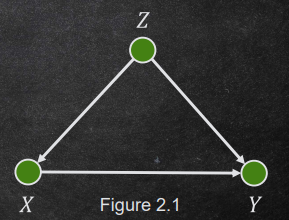
\includegraphics[width=0.35\textwidth]{img/confounding.png}
    \caption{Confounding effect of the covariate $Z$}
    \label{fig:confounding}
\end{figure}

We can consider average treatment effect equal to the associational difference
assuming the \textbf{ignorability} assumption.
\begin{definition}[Ignorability]
    The \textbf{ignorability} assumption states that the treatment assignment
    is random and independent of the potential outcomes:
    \begin{equation}
        Y(0), Y(1) \perp X
    \end{equation}
\end{definition}

Another name for this property is \textbf{exchangeability} because it can be
interpreted as we can exchange the groups can be exchanged without changing the
distribution of the potential outcomes.

We can distinguish between two types of ignorability: Mean ignorability and Full
ignorability. In general, mean ignorability is enough to compute the average
treatment effect.

This property is fundamental because it allows us to compute the average treatment
effect as the associational difference:
\begin{equation*}
    \tau \triangleq \mathbb{E}[Y(1) - Y(0)] = \mathbb{E}[Y|X = 1] - \mathbb{E}[Y|X = 0]
\end{equation*}

The assumption of ignorability allow us to identify causal effects. This can be
done reducing a causal expression to a purely statistical expression. We can
calculate the causal effect from just the observational distribution $P(X, Y, Z)$.

\begin{definition}[Identifiability]
    A causal quantity is identifiable if we can compute it from a purely statistical
    quantity.
\end{definition}

Unfortunately, the assumption of ignorability is completely unrealistic, confounding
is likely to happen in most data we observe. We can make the assumption of ignorability
more realistic by performing a \textbf{randomized experiment}.

In observational data, it's unrealistic to assume that the groups are exchangeable.
However, if we control for relevant variables by conditioning, then maybe the groups
will be exchangeable.

\begin{definition}[Conditional exchangeability]
    The \textbf{conditional exchangeability} or \textbf{unconfoundeness} assumption
    states that the treatment assignment is the potential outcomes conditional
    on the covariates:
    \begin{equation}
        Y(0), Y(1) \perp X | Z
    \end{equation}
\end{definition}

Indeed, when conditioning on $Z$, non-causal associations between $X$ and $Y$ no
longer exists. Non-causal association is blocked by conditioning on $Z$.

This is the main assumption necessary for causal inference. We can now identify
the causal effect within levels of $Z$, just like we did with ignorability:
\begin{equation}
    \mathbb{E}[Y(1) - Y(0) | Z] = \mathbb{E}[Y(1)| Z] - \mathbb{E}[Y(0)| Z] =
    \mathbb{E}[Y|X = 1, Z] - \mathbb{E}[Y|X = 0, Z]
\end{equation}

If we want the marginal effect that we had before when assuming ignorability, we
can get that by simply marginalizing over $Z$ as follows:
\begin{equation}
    \mathbb{E}[Y(1) - Y(0)] = \mathbb{E}_Z[\mathbb{E}[Y(1) - Y(0) | Z]]
\end{equation}

\begin{definition}[Adjustment formula]
    Given the assumption of unconfoundeness, positivity, consistency, and no interference,
    we can identify the average treatment effect as:
    \begin{equation}
        \tau = \mathbb{E}[Y(1) - Y(0)] = \mathbb{E}_Z[\mathbb{E}[Y(1) - Y(0) | Z]]
        = \mathbb{E}_Z[\mathbb{E}[Y|X = 1, Z] - \mathbb{E}[Y|X = 0, Z]]
    \end{equation}
\end{definition}

There may be some unobserved confounders that we can't control, this mean that
the assumption of unconfoundeness is violated. The best we can do is to observe
and fit as many covariates as possible to try to ensure unconfoundeness.

Indeed, it can be the case we obtain more biased estimates by including when
adjusting for the "wrong" covariates.

\begin{definition}[Positivity]
    Positivity is the condition that all the subgroups af the data with different
    value $z$ for covariates $Z$ have some probability of receiving treatment $X$.

    For all values $z$ of covariates $Z$ present in the population of interest,
    we have:
    \begin{equation}
        0 < P(X = 1 | Z = z) < 1
    \end{equation}
\end{definition}

If we have positivity violation, then we will be conditioning on a zero probability
event. This will lead to biased estimates.

Positivity is also referred to as the \textbf{overlap} assumption. This is because
we want the covariates distribution of the group to overlap.

\begin{figure}[!ht]
    \centering
    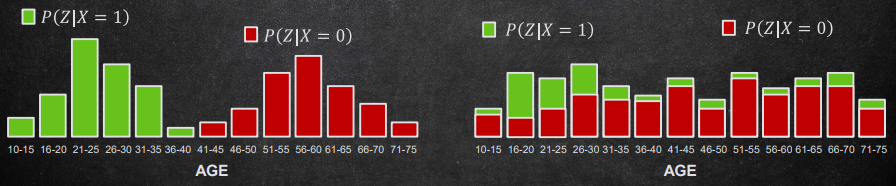
\includegraphics[width=\textwidth]{img/overlap.png}
    \caption{Example of overlap}
    \label{fig:positivity}
\end{figure}

Adjusting on more covariates can lead to curse of dimensionality.

Another important assumption is the \textbf{no interference} assumption. This
\begin{definition}[No interference]
    The outcome $Y_i$ of the $i^{th}$ individual is not affected by anyone else's
    treatment $X_j$ for $j \neq i$.
    \begin{equation}
        Y_i(x_1, x_2, \ldots, x_i, \ldots, x_n) = Y_i(x_i)
    \end{equation}
\end{definition}

The last assumption is the \textbf{consistency} assumption.
\begin{definition}[Consistency]
    If the treatment is $X$, then the observed outcome $Y$ is the potential outcome
    under treatment $X$. Formally:
    \begin{equation}
        X = x \rightarrow Y = Y(X)
    \end{equation}
\end{definition}

\begin{definition}[Stable Unit Treatment Value Assumption]
    The \textbf{Stable Unit Treatment Value Assumption} (SUTVA) is satisfied if
    individual $i$'s outcome $Y_i$ is simply a function of the treatment $X_i$.
\end{definition}

Now, we need to introduce some terminology that will be useful in the following
chapters.
\begin{itemize}
    \item \textbf{Estimand}: The quantity that we want to estimate.
    \item \textbf{Estimate}: an approximation of the estimand, which we get
          using data.
    \item \textbf{Estimator}: a function that maps the data to an estimate of the
          estimand.
    \item \textbf{Estimation}: the process that we use to go from data plus the
          estimand to a concrete number is known as estimation.
    \item \textbf{Causal estimand}: refers to any estimand that contains a potential
          outcome in it.
    \item \textbf{Statistical estimand}: refers to any estimand that does not contain
          a potential outcome in it.
\end{itemize}

The process of estimation is shown in figure \ref{fig:pipeline}. We need to
introduce also the concept of \textbf{identification}, which is the process of
moving a causal estimand to an equivalent statistical estimand. And the concept
of \textbf{Estimation}, which is the process of moving from a statistical estimand
to an estimate.
\begin{figure}[!ht]
    \centering
    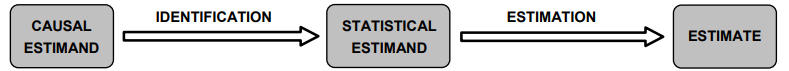
\includegraphics[width=\textwidth]{img/process.png}
    \caption{Process of estimation}
    \label{fig:pipeline}
\end{figure}